\section{STEADY-STATE THERMAL ANALYSIS}
\normalsize{Steady-state thermal analysis is the main type of analysis that was carried out to analyse the different components of the \acrshort{ECRH} \acrshort{TZM}-reflector tile assembly. Different scenarios and loadcases were designed to give insight on the thermal behavior and performances of the tile, that being, the impact of the design changes of the \acrshort{TZM}-reflector tile, the influences of different \acrshort{ECRH} beam configurations or the influences of the film coefficient in the cooling pipe.}
\subsection{Calculation of the surface integrales}
\normalsize{To compare between the old and new tile design but also validate the finite element model, calculating the surface integral can be of use. This idea behind this is to check for energy conservation after integration the heat flux of the \acrshort{ECRH} beam on the tile surface. Analytical calculations are a good approach to estimate the overall heat flow through the \acrshort{TZM} tile. After the calculation of the surface integrales ($\it{see}$ \ref{MODELLING OF THE ECRH BEAM}), it is possible to numerically estimate an integral and predictict the heat flux through the old and the new design.}
\\
\break
\normalsize{\indent The surface onto which the heat disribution is integrated is a rough approximation of the surface of the \acrshort{TZM} tile (the projected area of the tile was simplified to a rectangle of size $95mm \times 95mm$). The function is then integrated using a Wolfram Mathematica\textsuperscript{\textregistered} script. To evaluate the validity of the analytical calculation, a finite element model including only the old and the new \acrshort{TZM} tile was developed to calculate the surface integral but using the finite element method. The idea is to compare both methods to estimate the heat flow. }
\\
\begin{figure}[h!]
    \label{fig_5_1} 
    \centering
    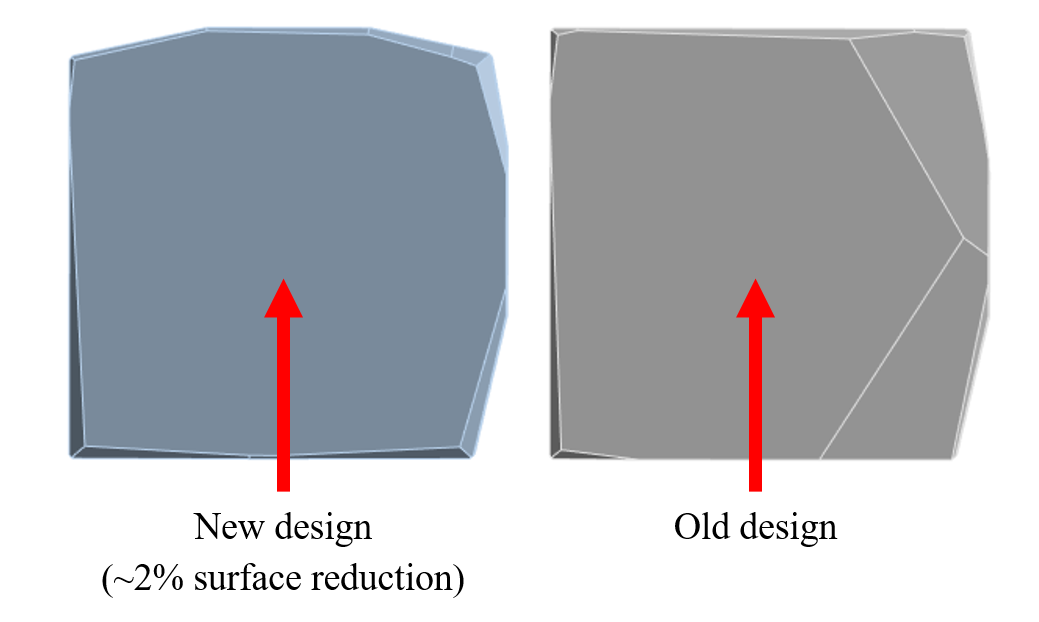
\includegraphics[width=.7\textwidth]{figures/standalonetilemodel.png}
    \caption{\it 3D model of the TZM tiles for integral calculation}
\end{figure}
\\
\break
\normalsize{\indent The idea of this analysis is to apply a heat flux on the plasma facing surface and a set temperature $(20 \si{\degree} C)$ at the back of the tile. This allows to calculate the power needed to assure $(20 \si{\degree} C)$ at the backside of the tile. According to the theory of conductivity, the heat flow entering the tile should be the same as the heat flow evacuated at the back. This can be calculated analytically using the integral form of Fourier's law. ($\it{see}$ \ref{HEAT CONDUCTION THEORY})}
\begin{equation}
    \oiint\displaylimits_{S} \ \mathbf{q} \cdot d \mathbf{S} \ = \ -k\oiint\displaylimits_{S} \ \mathbf{\nabla} T \cdot d \mathbf{S}
    % q_x \ = \ -k \ \partial_x T
    \tagaddtext{[\si{\watt}]}
    \label{eqn:IntFormofFourier}
\end{equation}
\\
\break
\normalsize{\indent The left hand side of the equation \refeq{eqn:IntFormofFourier} is the thermal power $\partial_t Q$ in [$W$] transferred by conduction and defined as $\partial_t Q \ \coloneqq \ \oiint_{S} \ \mathbf{q} \cdot d \mathbf{S}$. The differential $d \mathbf{S}$ is an oriented surface area element in [$m^2$]. On the right hand side of the equation is surface integral of the dot product between the temperature gradient $\mathbf{\nabla} T$ and an oriented surface area element $d \mathbf{S}$. To integrate this equation, it is assumed that the material is homogeneous with constant thermal conductivity. It is then possible to integrate \refeq{eqn:IntFormofFourier} for a 1-D geometry between two points. The result of the integration gives the following expression for heat flow expression:}
\begin{equation}
    %\oiint_{S} \ \mathbf{q} \cdot d \mathbf{S} \ = \ -k\oiint_{S} \ \mathbf{\nabla} T \cdot d \mathbf{S}
    \partial_t Q \ = \ -k \frac{A}{L} \Delta T
    \tagaddtext{[\si{\watt}]}
    \label{eqn:HeatFlow}
\end{equation}
\\
\break
\normalsize{\indent In this expression, $A$ is the cross-sectionnal area perpendicular to the heat flux in [$W$], $L$ is the distance between the two surfaces in [$m$], $\Delta T$ is the temperature difference between both front and back surfaces and $k$ is the thermal conductivity of the medium in [$W/m^2K$]. The cross-sectionnal area $A$ and the length $L$ are assumed constant as well as the thermal conductivity $k$. It is possible to determine the heat flow flowing through the tile and the heat flow evacuated through the boundary condition, they should be equal to satisfy energy conservation. Based on this, it is possible to use a model to approximate the heat flow through the tile.}
\\
\begin{figure}[h!]
    \label{fig_5_2} 
    \centering
    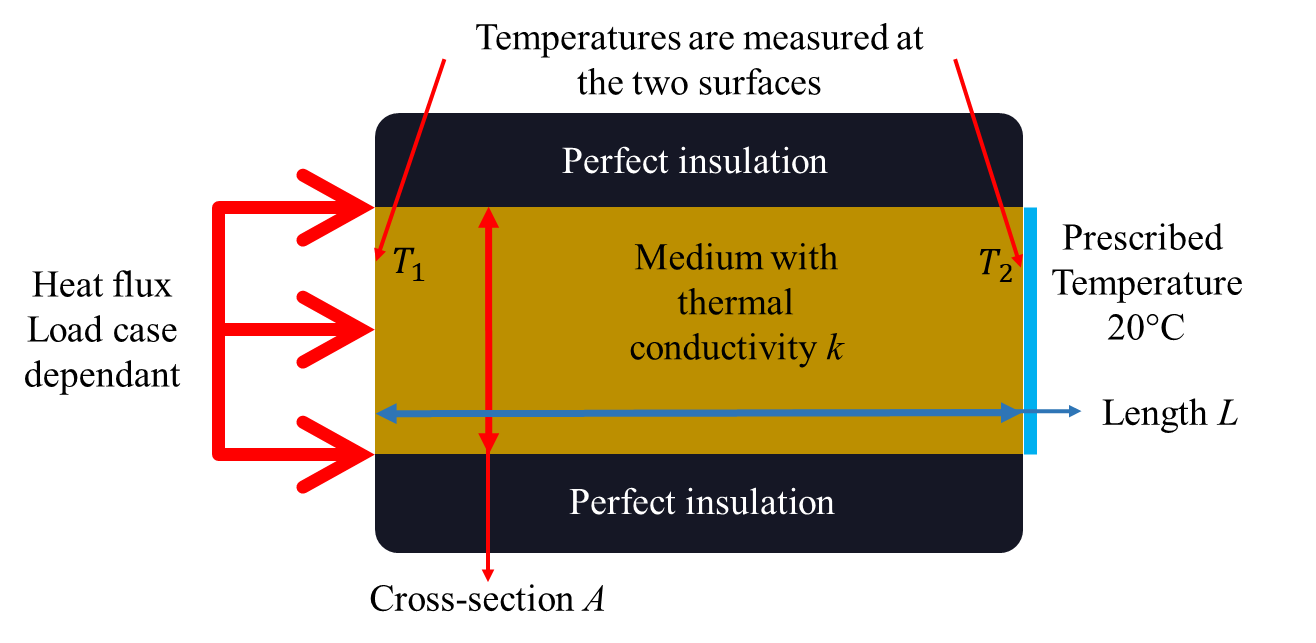
\includegraphics[width=.9\textwidth]{figures/modelforFEcalculationofsurfaceintegral.png}
    \caption{\it Model of the 1-D conduction test}
\end{figure}
\\
\break
\normalsize{\indent According to \refeq{eqn:HeatFlow}, the evolution of the temperature inside the medium is linear. It is then possible to calculate the heat flow flowing in and out (resp. $\partial_t Q_{in}$ and $\partial_t Q_{out}$). The idea is to find what heat flow $\partial_t Q_{out}$ is needed in order to respect the prescribed temperature boundary condition. After some calculations, it was found that $\partial_t Q_{in} \ = \ - \partial_t Q_{out}$. This validates the idea of calculating the surface integral using ANSYS\textsuperscript{\textregistered}. The solver settings of the ANSYS\textsuperscript{\textregistered} project are by default progam controlled. Since the calculation isn't too complex, it is acceptable to continue with these settings. Prescribed temperatures at the back of the \acrshort{TZM} tiles were defined and set to $20 \si{\degree} C$ (it is also important to keep in mind that the backside temperature doesn't affect the value of the integrales, any arbitrary temperature will work).}
\\
\begin{figure}[h!]
    \label{fig_5_3} 
    \centering
    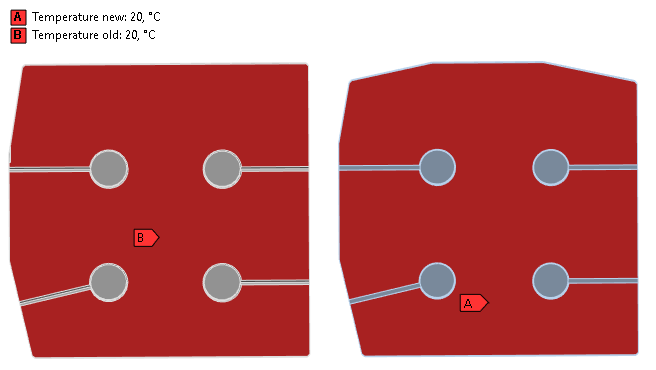
\includegraphics[width=1\textwidth]{figures/surfaceintegraleansysTEMPBC.png}
    \caption{\it Prescribed temperature of the ANSYS\textsuperscript{\textregistered} model for surface integral calculations}
\end{figure}
\\
\break
\normalsize{\indent The loadcases are the standard loadcases chosen to analyse the tile assembly. They are }
\\
\break
\newpage



\newpage
\begin{table*}\centering
\ra{1.3}
\begin{tabular}{@{}rrrrcrrrcrrr@{}}\toprule
& \multicolumn{3}{c}{$w = 8$} & \phantom{abc} & \multicolumn{3}{c}{$w = 16$}\\
\cmidrule{2-4} \cmidrule{6-8}
& $t=0$ & $t=1$ & $t=2$ && $t=0$ & $t=1$ & $t=2$\\ \midrule
$dir=1$\\
$c$ & 0.0790 & 0.1692 & 0.2945 && 0.3670 & 0.7187 & 3.1815\\
$c$ & -0.8651& 50.0476& 5.9384&& -9.0714& 297.0923& 46.2143\\
$c$ & 124.2756& -50.9612& -14.2721&& 128.2265& -630.5455& -381.0930\\
$dir=0$\\
$c$ & 0.0357& 1.2473& 0.2119&& 0.3593& -0.2755& 2.1764\\
$c$ & -17.9048& -37.1111& 8.8591&& -30.7381& -9.5952& -3.0000\\
$c$ & 105.5518& 232.1160& -94.7351&& 100.2497& 141.2778& -259.7326\\
\bottomrule
\end{tabular}
\caption{Caption}
\end{table*}


\subsection{Comparison between old and new TZM tile design}
\subsection{Film coefficient influence on thermal behavior}
\subsection{Loadcase influence on thermal behavior}